\documentclass[tikz,border=10pt]{standalone}
\usepackage{amsmath,amssymb}
\usetikzlibrary{positioning,arrows.meta,calc,fit,backgrounds}
\definecolor{tr}{HTML}{2E5EAA}
\definecolor{te}{HTML}{C8641E}
\definecolor{pr}{HTML}{2E8B57}
\begin{document}
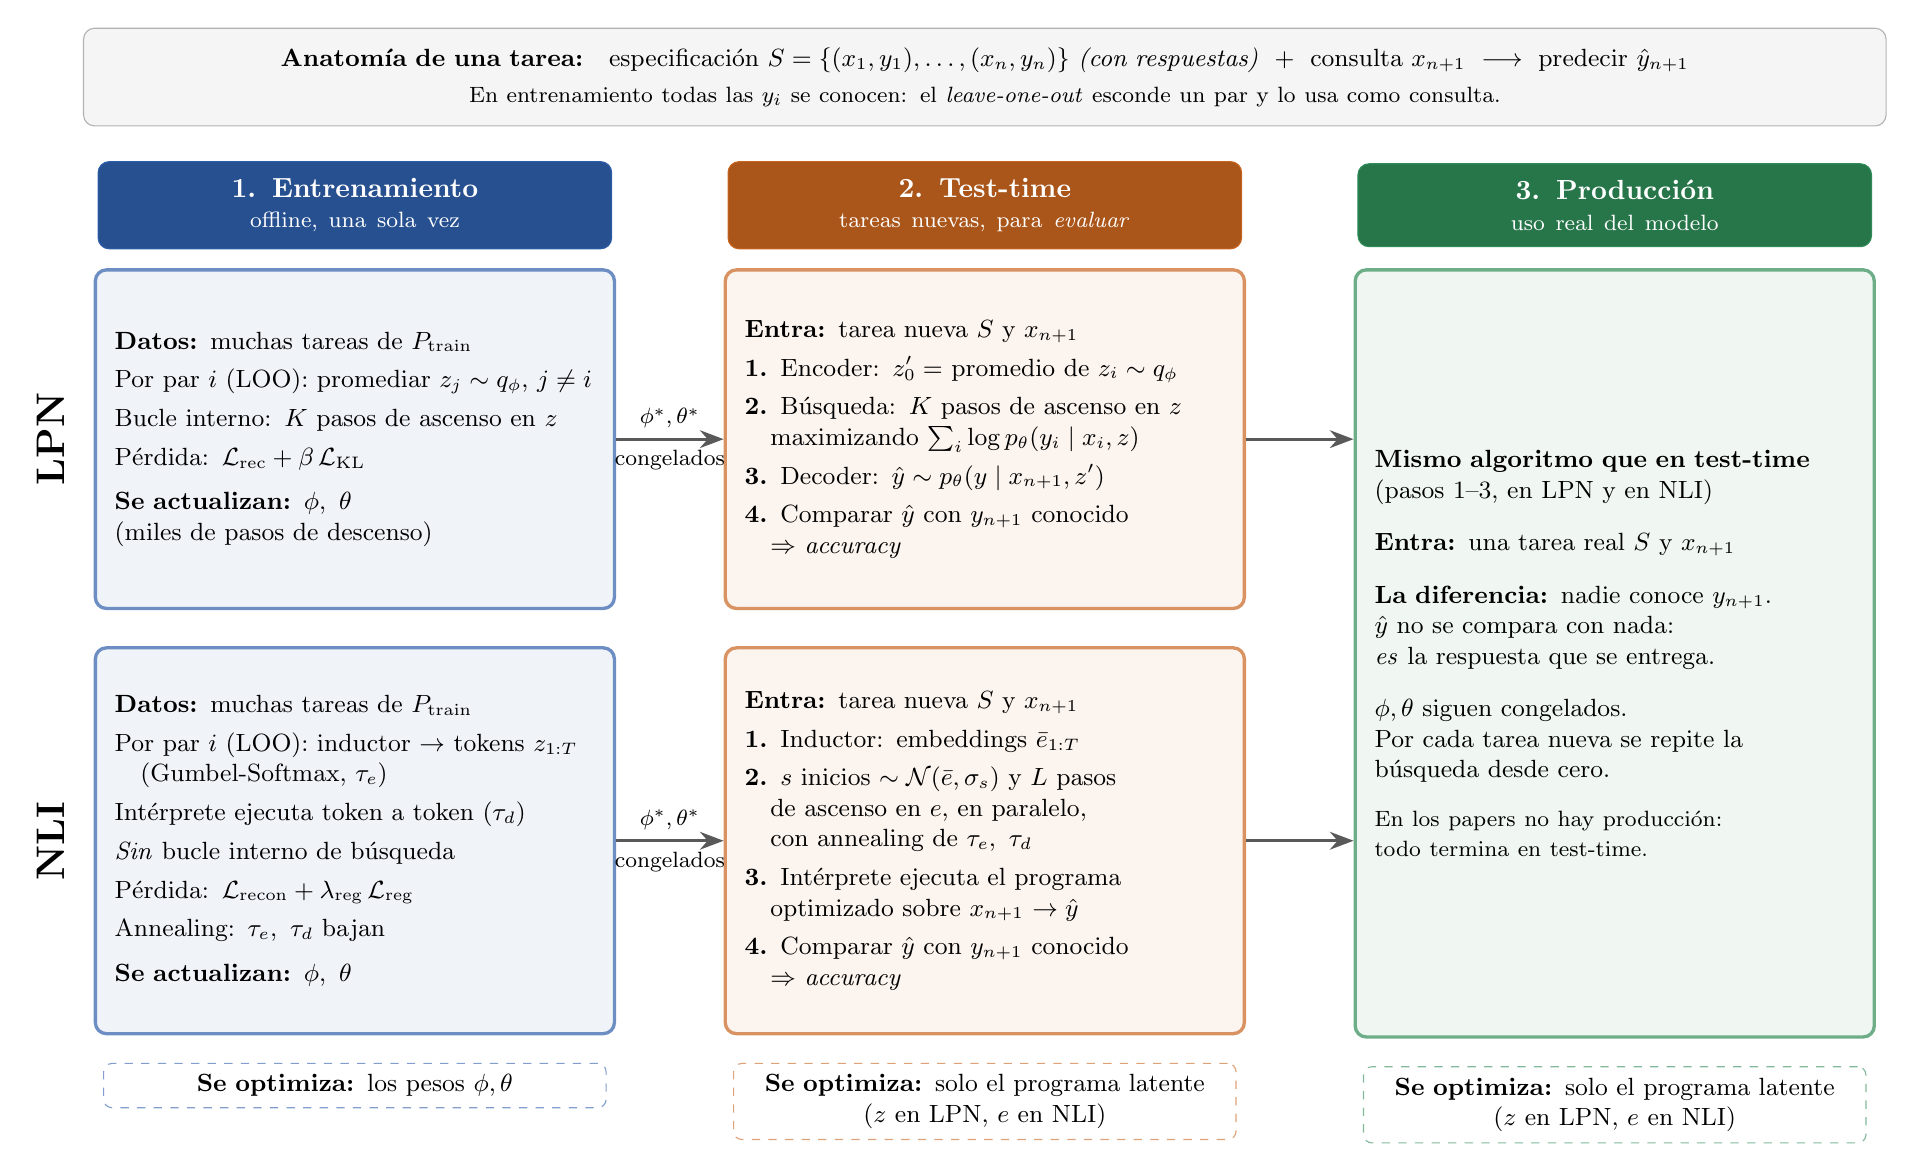
\begin{tikzpicture}[
  font=\small,
  head/.style={rounded corners=4pt, draw=#1, fill=#1!85!black, text=white,
               text width=6.1cm, align=center, inner sep=6pt, font=\bfseries},
  cell/.style={rounded corners=4pt, draw=#1!70, fill=#1!7, very thick,
               text width=6.1cm, align=left, inner sep=7pt, anchor=north},
  opt/.style={rounded corners=3pt, draw=#1!60, fill=white, dashed,
              text width=6.1cm, align=center, inner sep=4pt, anchor=north},
  rowlbl/.style={font=\Large\bfseries, rotate=90, anchor=south},
  arr/.style={-{Stealth[length=3mm]}, very thick, gray!70!black},
]
\def\cx{0} \def\cy{8.0} \def\cz{16.0}
\def\width{6.0}

% ---------- Anatomía de una tarea ----------
\node[rounded corners=4pt, draw=gray!60, fill=gray!8, text width=22.4cm,
      align=center, inner sep=7pt, anchor=south] (task) at (\cy,1.0)
  {\textbf{Anatomía de una tarea:}\quad
   especificación \mbox{$S=\{(x_1,y_1),\dots,(x_n,y_n)\}$} \emph{(con respuestas)}
   \;+\; consulta $x_{n+1}$ \;$\longrightarrow$\; predecir $\hat y_{n+1}$\\[2pt]
   \footnotesize En entrenamiento todas las $y_i$ se conocen: el \emph{leave-one-out}
   esconde un par y lo usa como consulta.};

% ---------- Encabezados ----------
\node[head=tr] (h1) at (\cx,0) {1. Entrenamiento\\[-1pt]\normalfont\footnotesize offline, una sola vez};
\node[head=te] (h2) at (\cy,0) {2. Test-time\\[-1pt]\normalfont\footnotesize tareas nuevas, para \emph{evaluar}};
\node[head=pr] (h3) at (\cz,0) {3. Producción\\[-1pt]\normalfont\footnotesize uso real del modelo};

% ---------- Fila LPN ----------
\node[cell=tr, minimum height=4.3cm] (l1) at (\cx,-0.8) {
  \textbf{Datos:} muchas tareas de $P_{\text{train}}$\\[3pt]
  Por par $i$ (LOO): promediar $z_j\sim q_\phi$, $j\neq i$\\[3pt]
  Bucle interno: $K$ pasos de ascenso en $z$\\[3pt]
  Pérdida: $\mathcal L_{\text{rec}}+\beta\,\mathcal L_{\text{KL}}$\\[5pt]
  \textbf{Se actualizan:} $\phi,\ \theta$ \\(miles de pasos de descenso)};
\node[cell=te, minimum height=4.3cm] (l2) at (\cy,-0.8) {
  \textbf{Entra:} tarea nueva $S$ y $x_{n+1}$\\[3pt]
  \textbf{1.} Encoder: $z'_0=$ promedio de $z_i\sim q_\phi$\\[3pt]
  \textbf{2.} Búsqueda: $K$ pasos de ascenso en $z$\\
  \quad maximizando $\sum_i\log p_\theta(y_i\mid x_i,z)$\\[3pt]
  \textbf{3.} Decoder: $\hat y\sim p_\theta(y\mid x_{n+1},z')$\\[3pt]
  \textbf{4.} Comparar $\hat y$ con $y_{n+1}$ conocido\\
  \quad $\Rightarrow$ \emph{accuracy}};

% ---------- Fila NLI ----------
\node[cell=tr, minimum height=4.9cm] (n1) at (\cx,-5.6) {
  \textbf{Datos:} muchas tareas de $P_{\text{train}}$\\[3pt]
  Por par $i$ (LOO): inductor $\to$ tokens $z_{1:T}$\\
  \quad (Gumbel-Softmax, $\tau_e$)\\[3pt]
  Intérprete ejecuta token a token ($\tau_d$)\\[3pt]
  \emph{Sin} bucle interno de búsqueda\\[3pt]
  Pérdida: $\mathcal L_{\text{recon}}+\lambda_{\text{reg}}\,\mathcal L_{\text{reg}}$\\[3pt]
  Annealing: $\tau_e,\ \tau_d$ bajan\\[5pt]
  \textbf{Se actualizan:} $\phi,\ \theta$};
\node[cell=te, minimum height=4.9cm] (n2) at (\cy,-5.6) {
  \textbf{Entra:} tarea nueva $S$ y $x_{n+1}$\\[3pt]
  \textbf{1.} Inductor: embeddings $\bar e_{1:T}$\\[3pt]
  \textbf{2.} $s$ inicios $\sim\mathcal N(\bar e,\sigma_s)$ y $L$ pasos\\
  \quad de ascenso en $e$, en paralelo,\\
  \quad con annealing de $\tau_e,\ \tau_d$\\[3pt]
  \textbf{3.} Intérprete ejecuta el programa\\
  \quad optimizado sobre $x_{n+1}$ $\to \hat y$\\[3pt]
  \textbf{4.} Comparar $\hat y$ con $y_{n+1}$ conocido\\
  \quad $\Rightarrow$ \emph{accuracy}};

% ---------- Producción (una celda para ambos) ----------
\path let \p1=(l2.north), \p2=(n2.south) in
  node[cell=pr, minimum height=\y1-\y2, text width=6.1cm] (p) at (\cz,\y1) {
  \textbf{Mismo algoritmo que en test-time}\\
  (pasos 1--3, en LPN y en NLI)\\[8pt]
  \textbf{Entra:} una tarea real $S$ y $x_{n+1}$\\[8pt]
  \textbf{La diferencia:} nadie conoce $y_{n+1}$.\\
  $\hat y$ no se compara con nada:\\
  \emph{es} la respuesta que se entrega.\\[8pt]
  $\phi,\theta$ siguen congelados.\\
  Por cada tarea nueva se repite la búsqueda desde cero.\\[8pt]
  \footnotesize En los papers no hay producción:\\
  \footnotesize todo termina en test-time.};

% ---------- Etiquetas de fila ----------
\node[rowlbl] at ($(l1.west)+(-0.25,0)$) {LPN};
\node[rowlbl] at ($(n1.west)+(-0.25,0)$) {NLI};

% ---------- Flechas ----------
\draw[arr] (l1.east) -- node[above, font=\footnotesize, black]{$\phi^*,\theta^*$}
                        node[below, font=\footnotesize, black]{congelados} (l2.west);
\draw[arr] (n1.east) -- node[above, font=\footnotesize, black]{$\phi^*,\theta^*$}
                        node[below, font=\footnotesize, black]{congelados} (n2.west);
\draw[arr] (l2.east) -- (l2.east -| p.west);
\draw[arr] (n2.east) -- (n2.east -| p.west);

% ---------- ¿Qué se optimiza? ----------
\node[opt=tr] (o1) at ($(n1.south)+(0,-0.35)$)
  {\textbf{Se optimiza:} los pesos $\phi,\theta$};
\node[opt=te] (o2) at ($(n2.south)+(0,-0.35)$)
  {\textbf{Se optimiza:} solo el programa latente\\($z$ en LPN, $e$ en NLI)};
\node[opt=pr] (o3) at ($(p.south)+(0,-0.35)$)
  {\textbf{Se optimiza:} solo el programa latente\\($z$ en LPN, $e$ en NLI)};
\end{tikzpicture}
\end{document}
